%%____________________________________________________________________________||
\section{Systematic uncertainties}
\label{sec:systematics}
This section addresses the estimation of systematic uncertainties in the analysis.
Since the detailed and complete study of the systematics can be meaningfully carried on only with the data, 
for the MC-based PHYS14 exercise presented in this note we rather intend to describe the strategy to compute them 
in data and present the assumptions made to get the projections of physics reach, which are detailed in Section \ref{sec:susy}. 

The uncertainties are divided in ``normalisation'' and ``shape'' systematics. \\
The first type affects the yields of the background in the signal region in each (\nb,\njet,\HT) 
category and is estimated through closure tests as described in section \ref{sec:bkgdnorm-syst}. \\
The bin-by-bin migration between \mht bins within the same \HT bin is taken into account implementing 
shape uncertainties, providing alternative template \mht shapes together with the nominal one.

% % Maybe we can re-use this table at some point
% \begin{table}[h!]
%   \caption{Systematic uncertainties on the transfer factors as a
%     function of \scalht.}  
%   \label{tab:bkgd-syst}
%   \setlength{\extrarowheight}{2.5pt}
%   \centering
%   \begin{tabular}{ llccc }
%     \hline
%     \hline
%     \scalht region [GeV] & 200-600 & 600-1000  & $>1000$  \\ 
%     \hline
%     Uncertainty [\%] & 10 & 20 & 30 \\
%     \hline
%     \hline
%   \end{tabular}
% \end{table}
%
% The uncertainties associated with the b-tag ``fomula method'' used
% during Run~1 are ascertained through a dedicated procedure and are
% assumed to be sub-dominant with respect to the \scalht-dependent
% uncertainties derived from the closure tests, as observed during
% Run~1. 
%\clearpage

\subsection{Closure tests and systematic uncertainties on transfer factors\label{sec:bkgdnorm-syst}}

The background yields are determined fn each of the (\nb,\njet,\HT) event category 
by defining transfer factors from control region to signal region, as described in \ref{sec:background}. 
Several sources of systematic uncertainties affect each factor, like 
theoretical uncertainties~\cite{Bern:2011pa}, 
limitations in the simulation modelling of event kinematics and
instrumental effects. This section describes how the systematic
uncertainties are assessed from closure tests in data.

\subsubsection{Closure tests\label{sec:closure-tests-desc}}

The sensitivity of the transfer factors to potential limitations in
the simulation modelling is established through sets of closure tests,
which confront data yields measured in one data control (sub-)sample
against the predictions determined from another data control
(sub-)sample as a function of \scalht. \ie, an extrapolation is made
from one control (sub-)sample to another (rather than to the signal
region) in bins of \scalht via appropriate transfer factors, again
determined from simulation. A large ensemble (\ie hundreds) of
statistically independent closure tests are performed between a number
of control (sub-)samples to identify any potential sources of bias in
the transfer factors.

The level of statistical consistency between the predicted and
observed yields of each closure test in the ensemble is inspected, in
the absence of any bias in the transfer factors. The level of
agreement between the predicted and observed yields is expressed as
the ratio $(\nobs - \npre)/\npre$ while considering only the
statistical uncertainties on \npre and \nobs. Therefore, the level of
closure is defined by the statistical significance of a deviation in
the ratio from zero. A set of closure tests comprise ratios determined
for each \scalht bin. In this way, a set of closure tests allow to
establish the presence of significant biases or otherwise, and any
possible dependence on \scalht. If statistically significant biases
are observed, further studies are required to understand and correct
for these biases.

Under the assumption of closure for the full ensemble of tests,
systematic uncertainties on the transfer factors are derived for each
\njet and \nb category and \scalht regions. The treatment for
estimating the systematic uncertainties on the transfer factors is
described in Section~\ref{sec:syst-from-closure}.

Thirteen sets of closure tests use the five data control samples to
probe key ingredients of the simulation modelling of the SM
backgrounds with genuine \met as a function of \scalht, as shown in
Fig.~\ref{fig:closure}. This is done for each jet multiplicity bin
separately. Results are shown for 4 and $\geq$ 5 jets for both 3 \ifb and 10 \ifb: 
%create mode 100644 notes/AN-15-004/trunk/figures/closureTests/summary_plots10fb.pdf
%create mode 100644 notes/AN-15-004/trunk/figures/closureTests/summary_plots1fb.pdf
%create mode 100644 notes/AN-15-004/trunk/figures/closureTests/summary_plots3fb.pdf
%create mode 100644 notes/AN-15-004/trunk/figures/closureTests/systOut2d10fb.pdf
%create mode 100644 notes/AN-15-004/trunk/figures/closureTests/systOut2d1fb.pdf
%create mode 100644 notes/AN-15-004/trunk/figures/closureTests/systOut2d3fb.pdf
\begin{figure}[h!]
  \begin{center}
    \subfigure[$\njet = 4$]{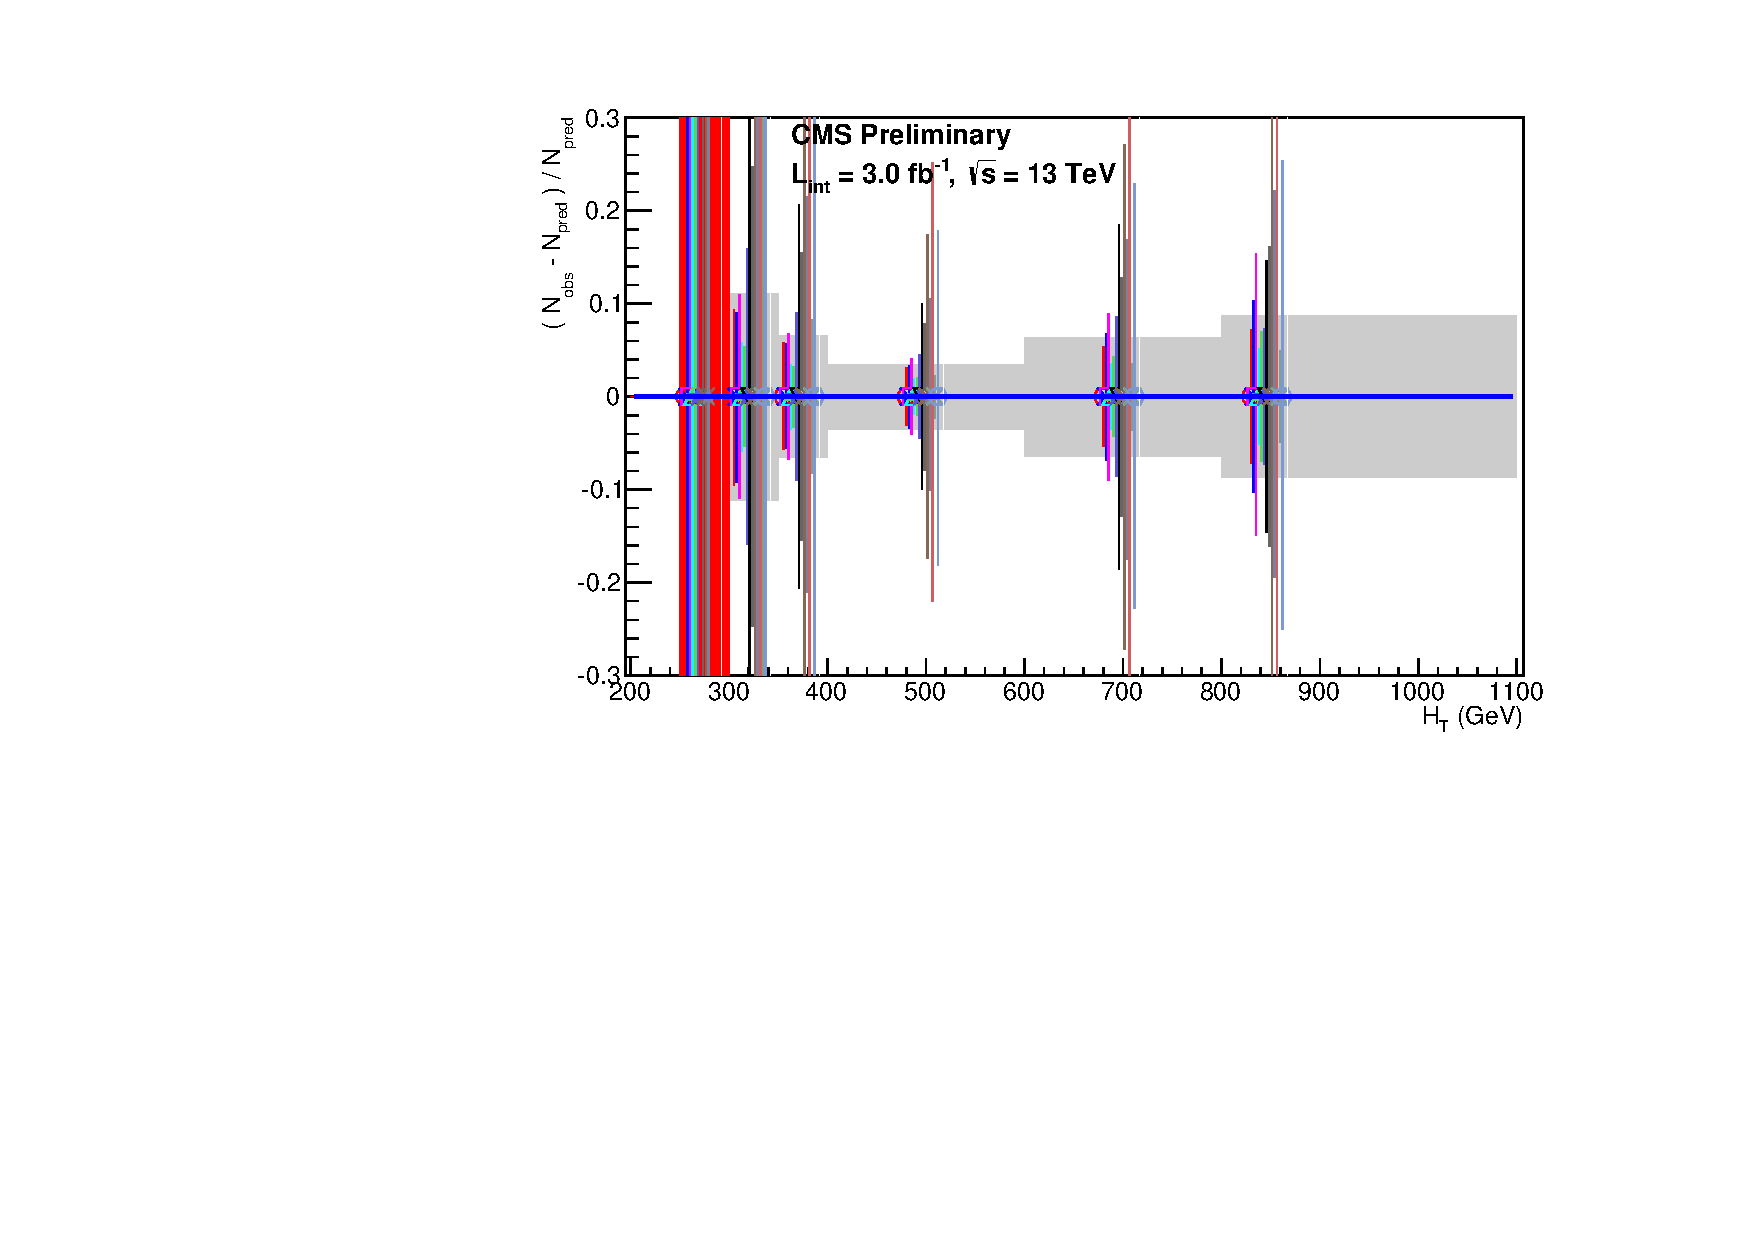
\includegraphics[width=0.5\textwidth]{figures/closureTests/eq4j_htClosure_3fb.pdf}} ~~
    \subfigure[$\njet \geq 5$]{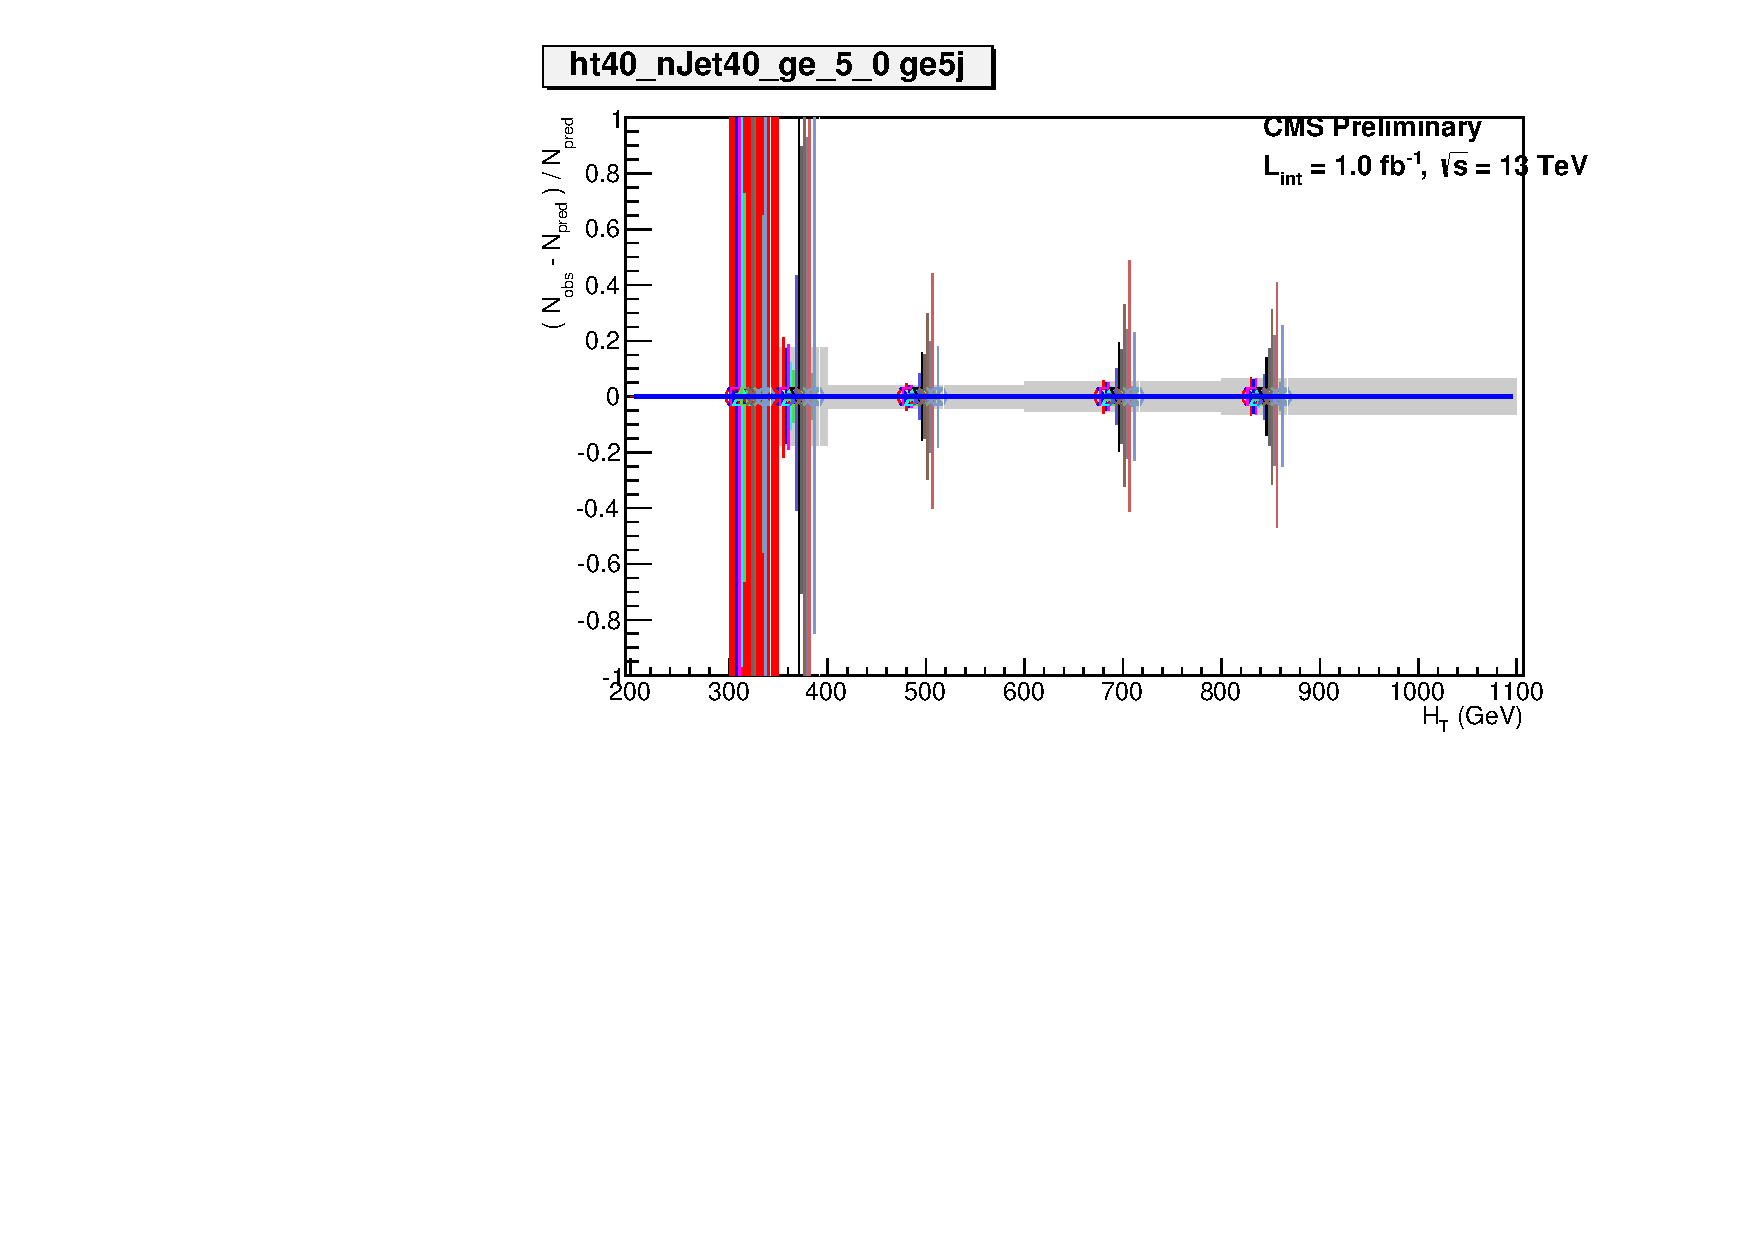
\includegraphics[width=0.5\textwidth]{figures/closureTests/ge5j_htClosure_3fb.pdf}} \\
    \subfigure[$\njet = 4$]{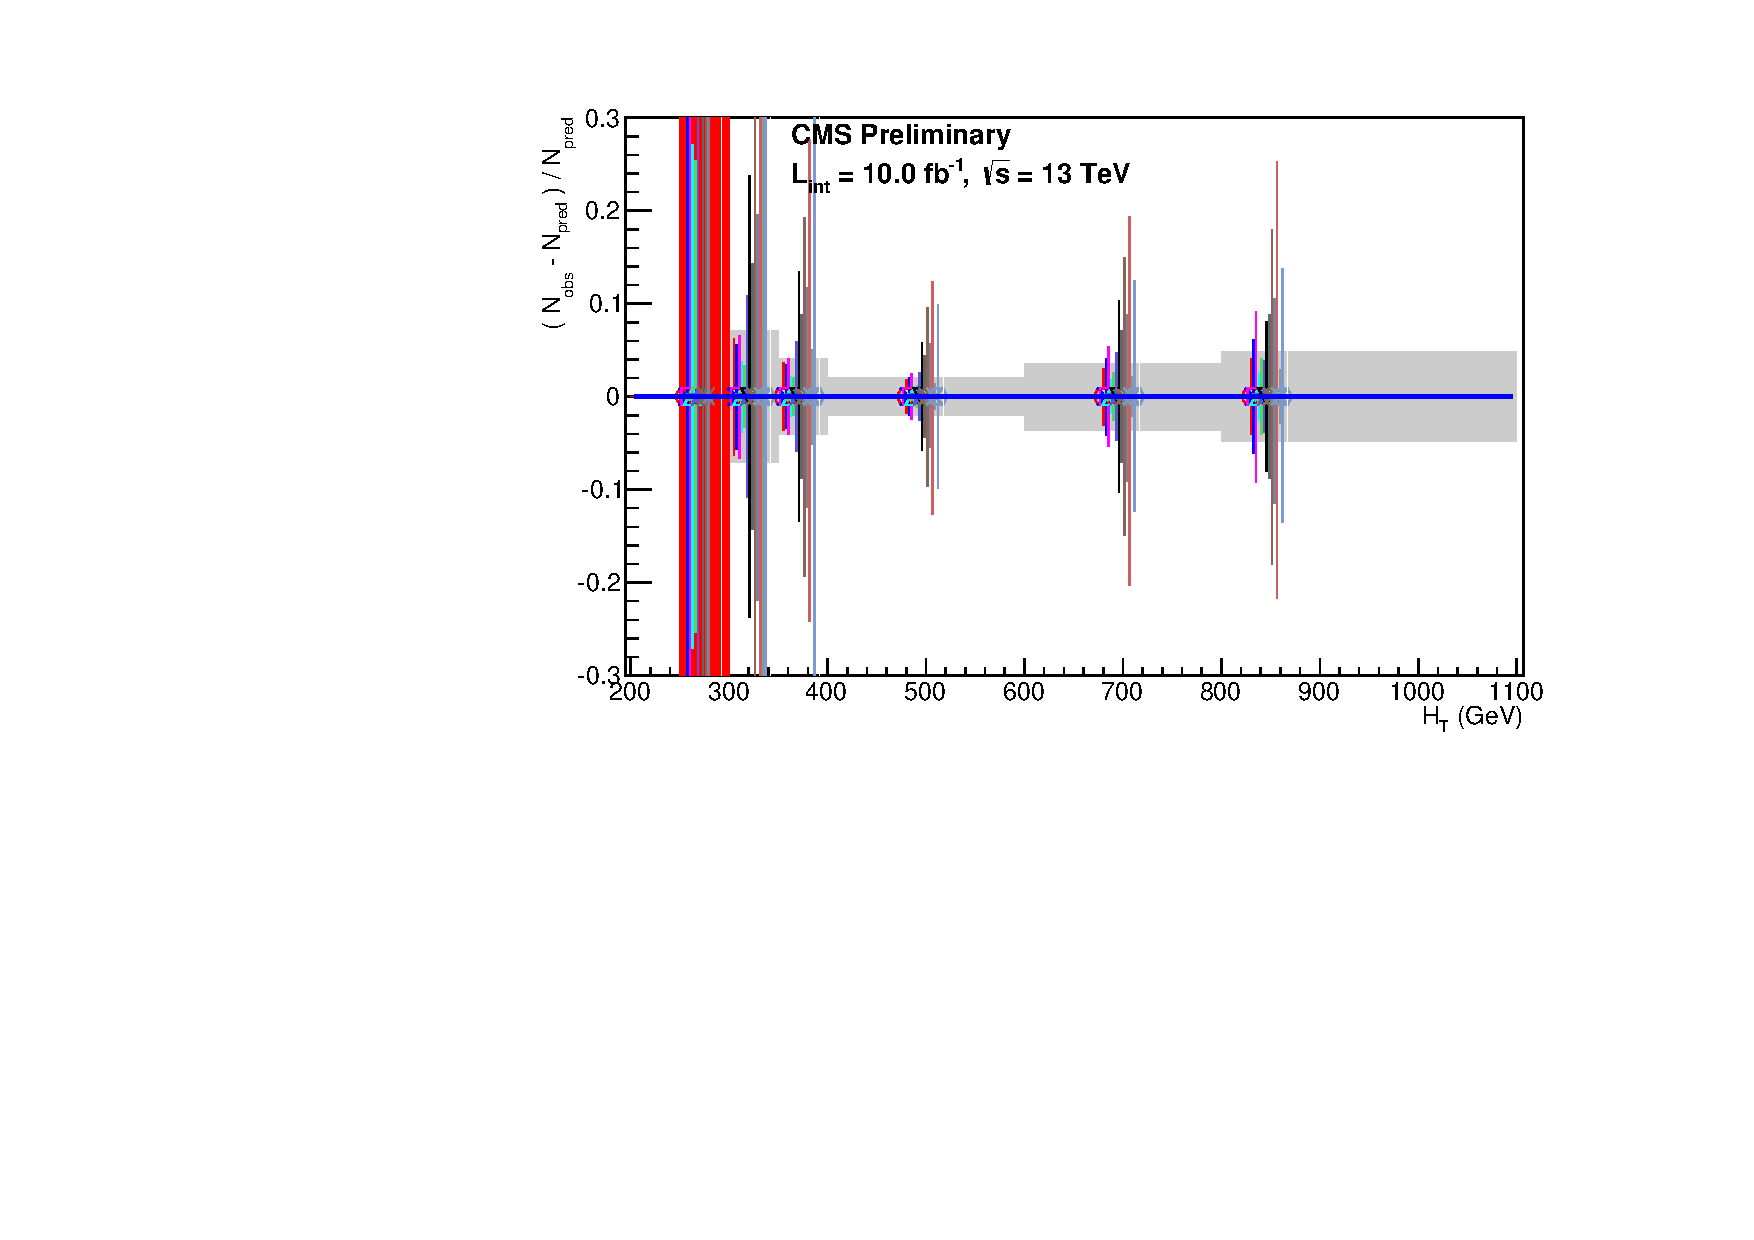
\includegraphics[width=0.5\textwidth]{figures/closureTests/eq4j_htClosure_10fb.pdf}} ~~
    \subfigure[$\njet \geq 5$]{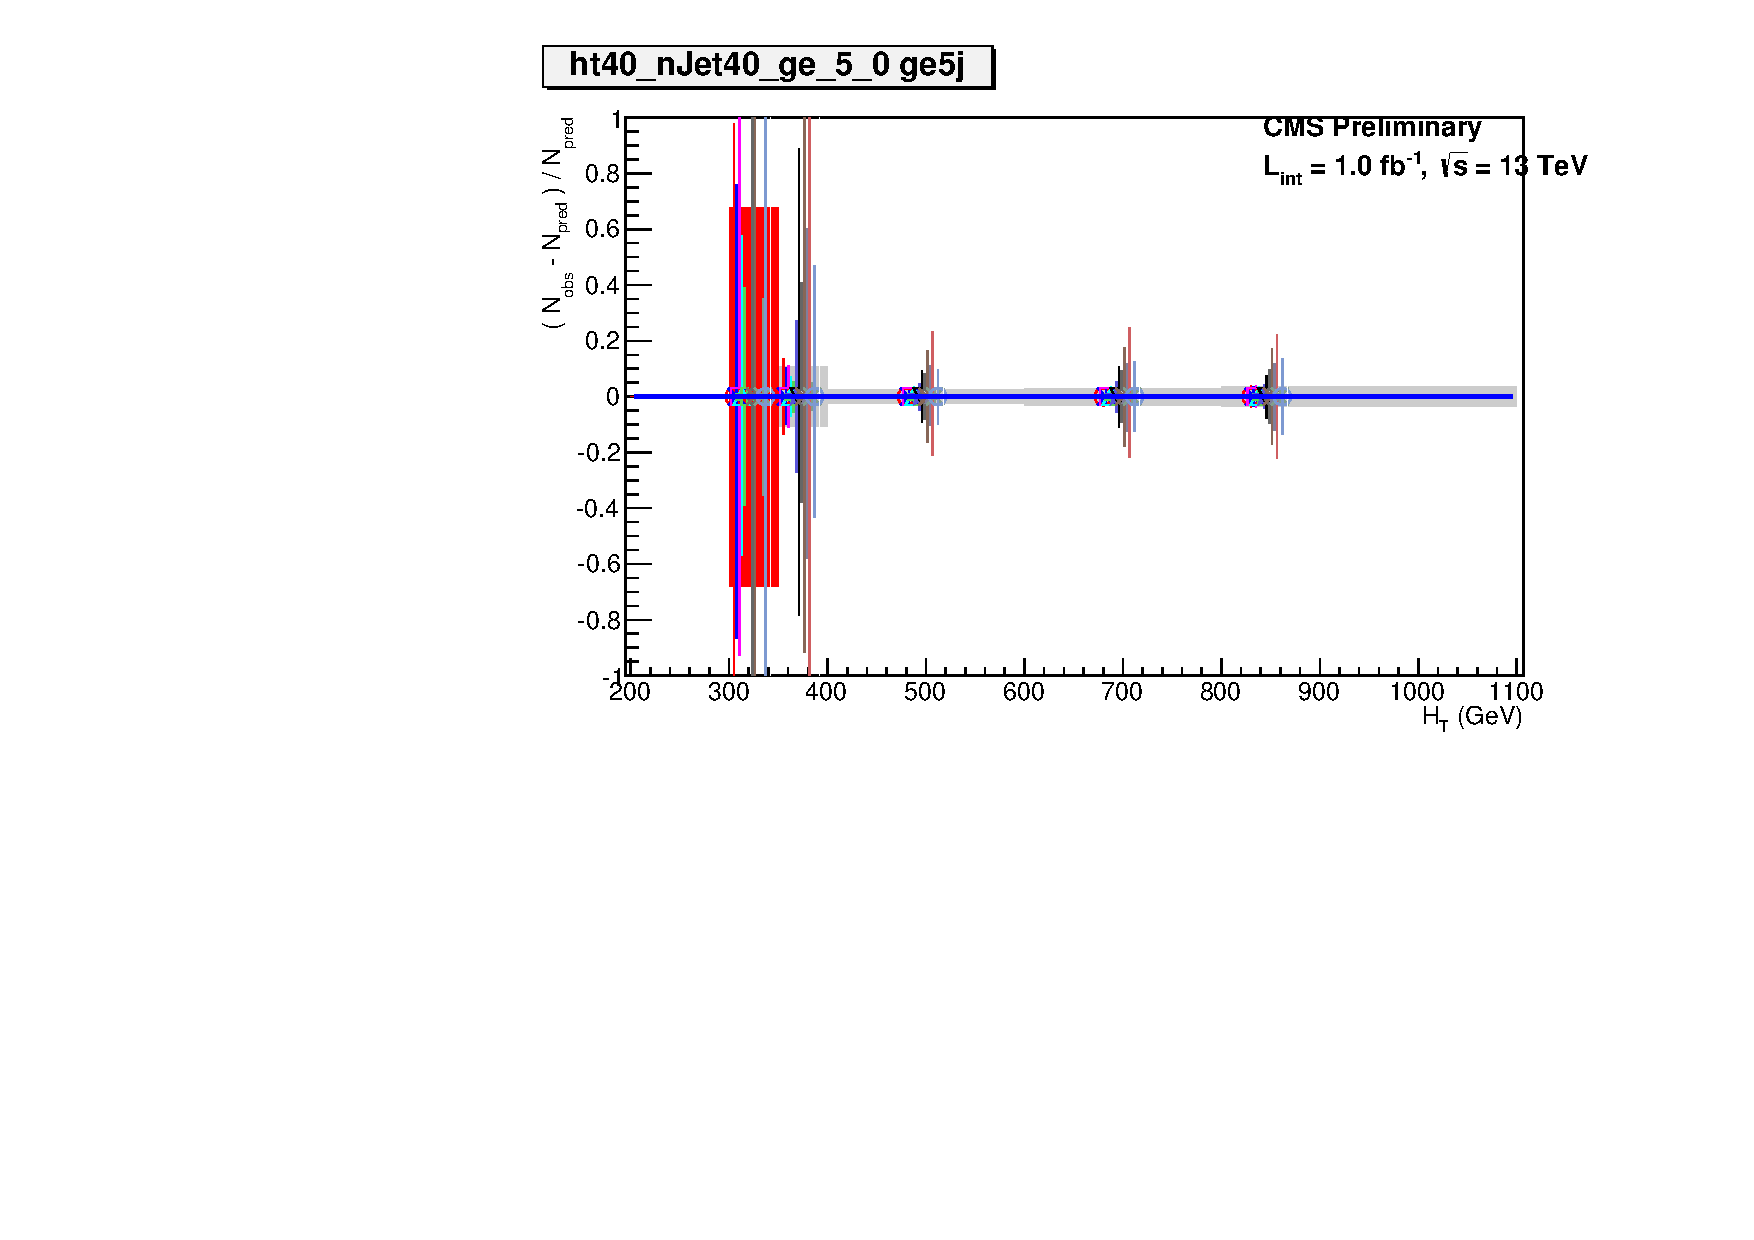
\includegraphics[width=0.5\textwidth]{figures/closureTests/ge5j_htClosure_10fb.pdf}} \\
    \caption{Sets of closure tests (open symbols) overlaid on top of
      the systematic uncertainty used for each of the seven \scalht
      bins (shaded bands) and for two different jet
      multiplicity bins: (a) $\njet = 4$ and (b) $\njet \geq5$.}
    \label{fig:closure}
  \end{center} 
\end{figure}

The first three sets of closure tests are carried out between the $\mu$ 
+ jets sample and the e + jets sample. These probe the lepton 
identification for three scenarios: 0 (red circles), 
1 (times symbols) and $\geq$2 (squares) b-tags, corresponding to samples with a different admixture of the $W$ and \ttbar processes., 
and, as a consequence, different kinematic. 
%% In particular, the 0 b-tag sub-sample is enriched in $W$+jets events, while the $\geq$2 b-tags is very pure in \ttbar.
% The first three sets of closure tests are carried out within the $\mu$
% + jets sample. The first set (indicated by circles) probes the
% modelling of the \alphat distribution in genuine \met events as a
% function of \scalht. This is important to verify the approach of using
% \mj and \mmj samples without an \alphat requirement to make background
% predictions in the signal region, as described in
% Sec.~\ref{sec:larger}. The tests confront data yields in the \mj
% sample with an \alphat requirement against predictions determined in a
% \mj sample with the \alphat requirement inverted. As usual,
% corresponding expectations from simulation are obtained to construct
% the transfer factors required to make the predictions.

The fourth (triangles) and fifth (green crosses) sets probe the
sensitivity of the transfer factors to the relative admixture of
events from the $W$ + jets and \ttbar processes. These tests are
extremely conservative, as the admixture changes little between the
\mj sample and the signal region, whereas the closure tests use
sub-samples with very different admixtures of W + jets and \ttbar
events. \eg, the former uses a W-enriched sub-sample (selected by
requiring zero b-jets) to predict yields in a \ttbar-enriched
sub-sample (selected by requiring one b-jet). 
These two tests also probe the modelling of the reconstruction of b-quark jets, 
although this can be addressed more precisely by dedicated studies, as the one 
performed in the previous analysis, see for instance \cite{CMS_AN_2013-366}.

The sixth (hollow stars) and seventh (inverse triangles) set deal 
with the consistency of the prediction of W + jets with $\gamma$ + jets.
This is useful in general for understanding the predictions of the \znunu + jets background from the \gj process. 

The eigth (diamonds) and ninth (brown asterix), connecting the $\mu$ + jets 
and $\mu\mu$ + jets control samples, again addresses the modelling of 
the relative contributions of $Z$ + jets to $W$ + jets and \ttbar events.
This set of tests is again a very conservative probe of the sensitivity of the
transfer factors to the W + jets and \ttbar admixture. At some
level, the muon trigger and reconstruction efficiencies are probed
too, given that exactly one and two muons are required in the two
control samples. However, dedicated data-driven methods are used to
measure the muon trigger and reconstruction efficiencies, with values
taken from the muon POG.

The tenth (solid stars) and eleventh (red crosses) deal  with the consistency between the
Z$\rightarrow ee$ + jets and $\gamma$ + jets samples, which is an
important self-consistency cross-check between two independent methods
used to predict the same irreducible background of \znunu + jets
events. Hence, this is also an important check on the validity of
using the \gj process to predict the \znunu\, + jets process.
%, for which a 20\% theoretical uncertainty on the ratio of
%cross-sections is assumed~\cite{PAS-SUS-08-002,Bern:2011pa}.

The twelth, and thirteenth tests probe the simulation modelling of
the jet multiplicity in the e + jets (green asterix), and ee + jets 
(blue circles), which is checked due to the exclusive binning in jet multiplicity.
As in the case of the W + jets / \ttbar admixture, this set of tests is a very 
conservative check, as predictions are always made from the same 
jet multiplicity bin, whereas the closure tests translate between the two bins.

% This section assumes data - must alter to what we show
In summary, each set of closure tests should demonstrate, within the
statistical precision of each test, that there are no significant
biases or dependencies on \scalht inherent in the transfer factors
obtained from simulation. To ensure this zero and first order polynomial
fits will be performed along the \scalht dimension for each closure test 
and jet category. The fits will be inspected for any indication of bias 
averaged over \scalht as well as a bias dependant on \scalht. 

\subsubsection{Systematic uncertainties from closure tests\label{sec:syst-from-closure}}

Once it is established that no significantly large bias or trend is
observed for any set of closure tests, the systematic uncertainties
are determined. The statistical precision of the closure tests is
considered a suitable benchmark for determining the systematic
uncertainties that are assigned to the transfer factors, as it is only
the statistical uncertainties associated with the tests that limit our
knowledge of whether closure is actually achieved or otherwise.

Systematics are determined for seven regions in \scalht,
for each jet category. In data, for each \scalht region, the systematic uncertainty 
is estimated by taking the quadrature sum of the weighted mean and sample variance for 
the closure tests within the given \scalht region. To find expected systematics \nobs and \npre are 
taken from the same Monte Carlo (guaranteeing closure) but the statistical errors are 
from the unweighted and weighted counts respectively. The expected systematic uncertainty is then 
taken as the weighted mean of the error on the closure tests. This is an estimator of the expected variance
assuming no bias that should be found in data. 
This procedure yields the values quoted in Figure~\ref{fig:systematics} for the statistics
dominated scenario (3 \ifb) and the systematics dominated scenario (10 \ifb). 
A missing entry implies that the statistics were insufficient to complete the 
necessary set of closure tests and the \scalht bin is not used for this jet category. 
In addition to the fits described in \ref{sec:syst-from-closure} comparing the 
size of the systematic found in data with that expected will provide 
an indication of any genuine bias.

The uncertainty related to the modelling of b-quark jets
in simulation on the transfer factors is studied separately and 
found to be very small, at the percent level, as discussed in Section~\ref{sec:btag-syst}. 
This source of uncertainty is however included in the closure tests described previously.
%% , in
%% comparison to the aforementioned \njet- and \scalht-dependent
%% systematic uncertainties.


Figure \ref{fig:systematics} shows the systematic uncertainty on the trasfer factor as a function of the \HT and (\nb,\njet) category, 
extracted with the procedure described above, as they are expected in the absence of bias (i.e. perfect closure).

\begin{figure}[]
  \centering
  \subfigure[Systematic uncertainties for the 3 \ifb luminosity scenario
  (luminosity 3 \ifb)]{
    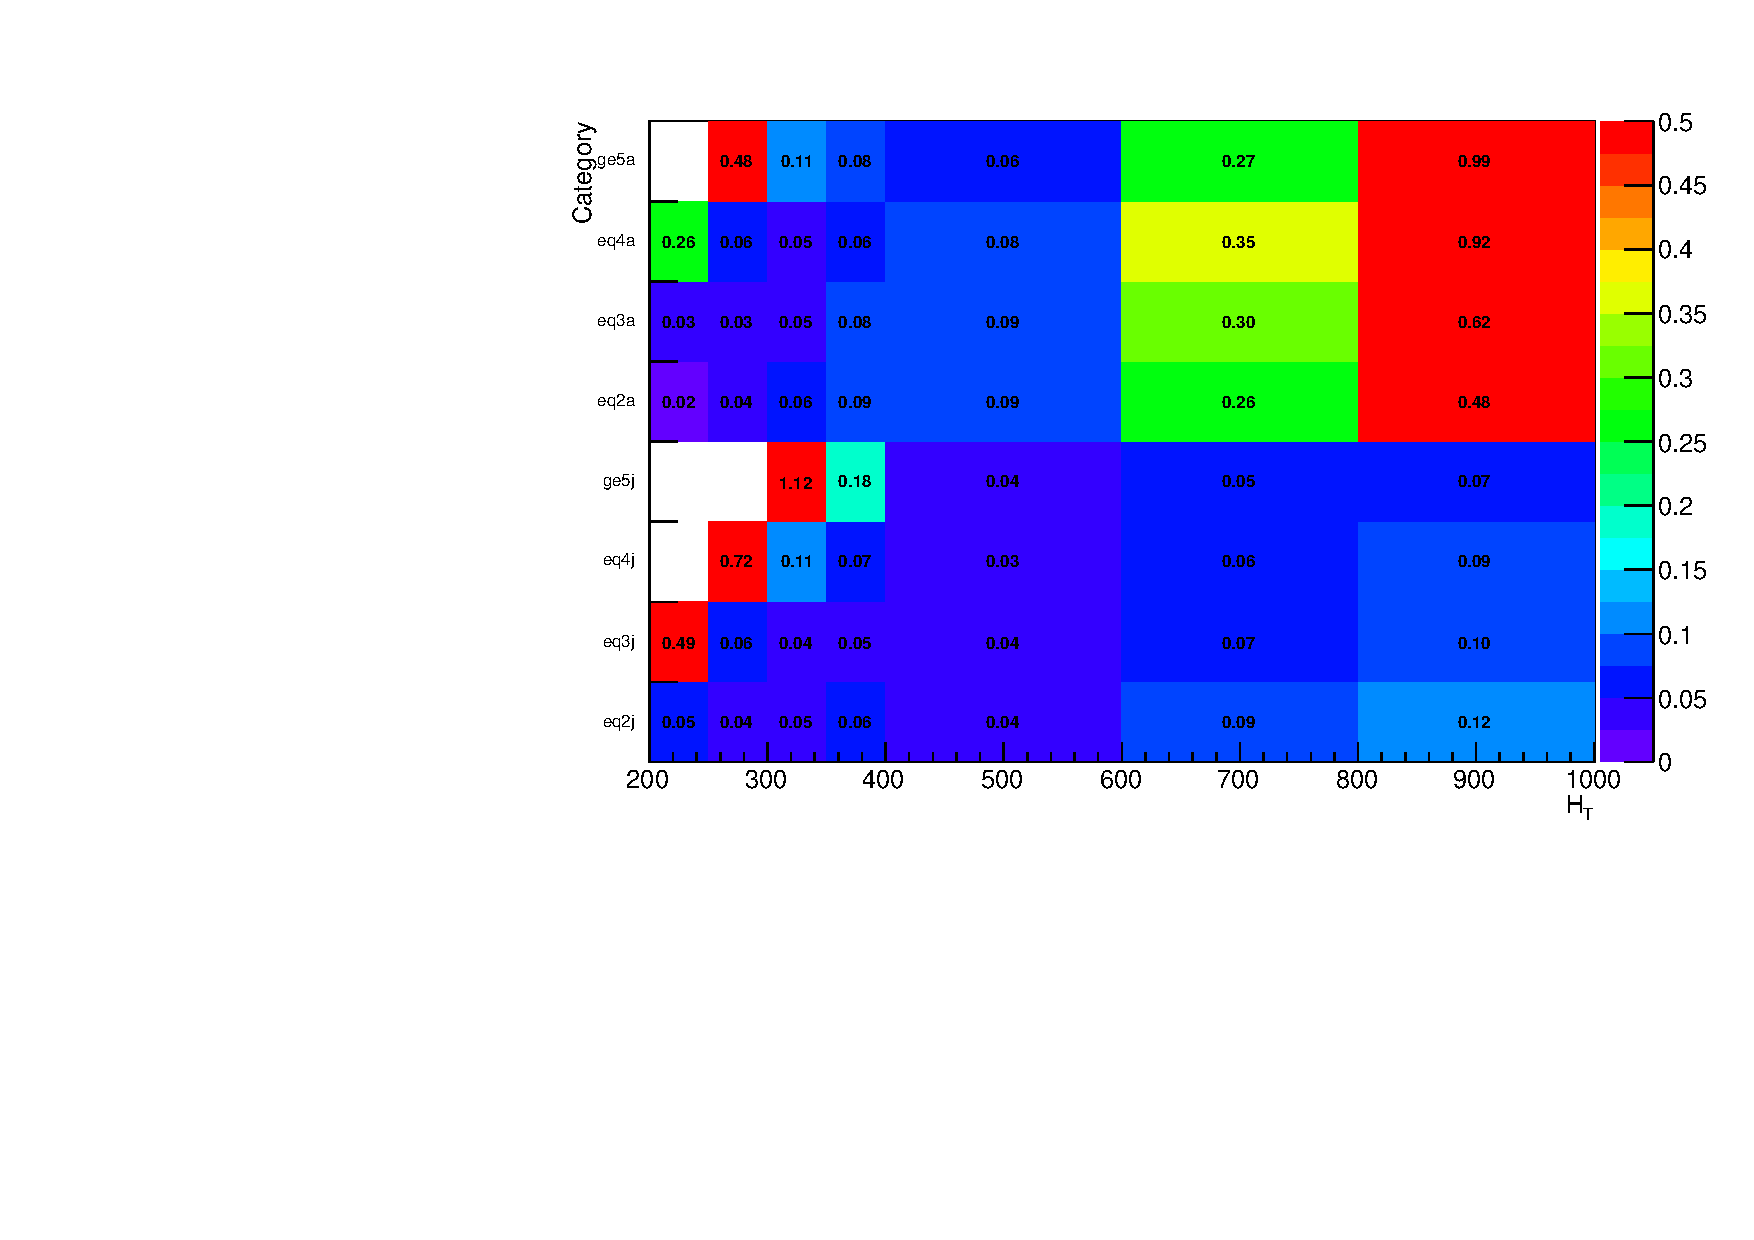
\includegraphics[width=0.5\textwidth]{figures/closureTests/systOut2d3fb.pdf}
  } ~~
  \subfigure[Systematic uncertainties for the 10 \ifb luminosity scenario
  (luminosity 10 \ifb)]{
    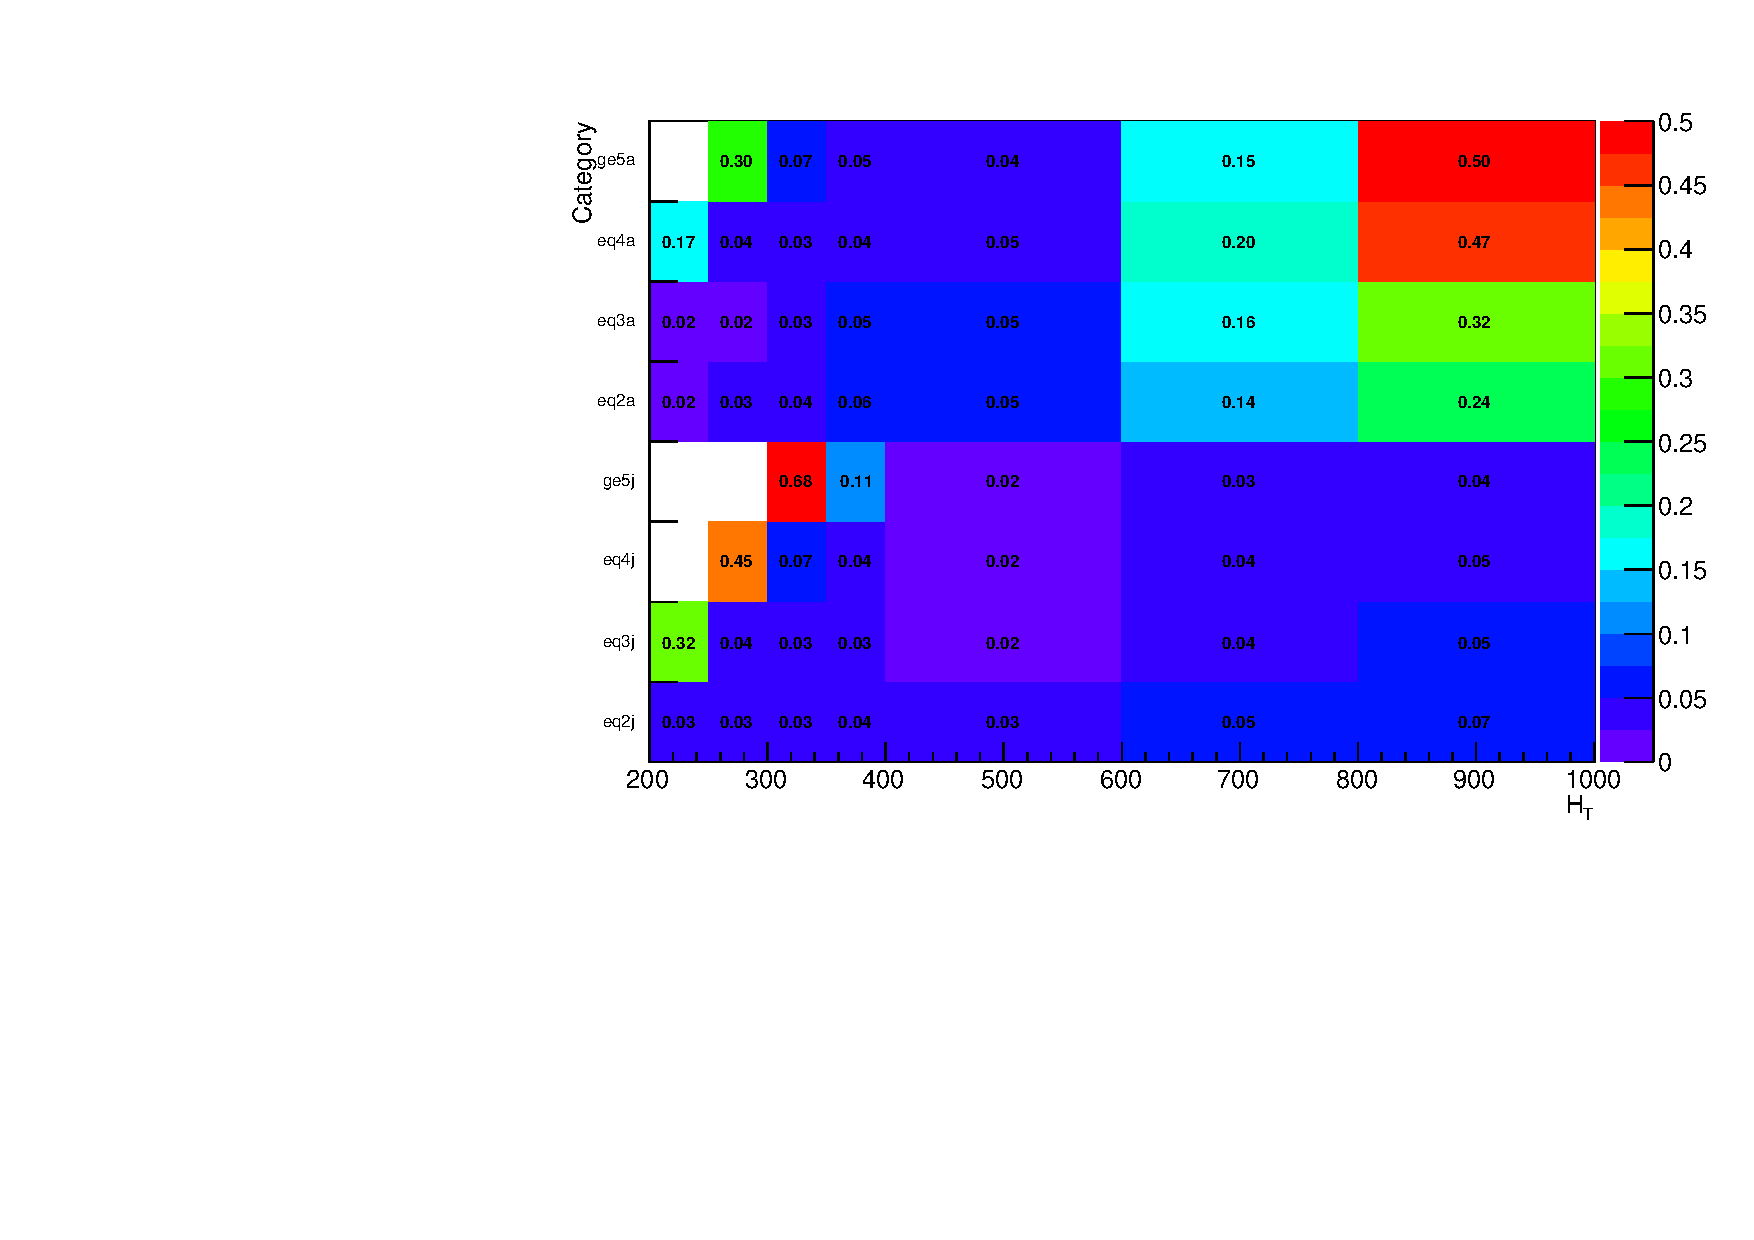
\includegraphics[width=0.5\textwidth]{figures/closureTests/systOut2d10fb.pdf}
  }
  \caption{\label{fig:systematics} Expected systematics derived from the closure tests shown for
the 3 \ifb and 10 \ifb scenarios}
\end{figure}

These systematic uncertainties are assumed to fully uncorrelated between the different 
event categories, as described in section \ref{sec:likelihood}. 
This is believed to be a conservative approach, given that one can expect some
correlation between adjacent \scalht bins (due to comparable
kinematics).

%% b jet multiplicity categories and also the seven \scalht regions,
%% which is a conservative approach given that one can expect some
%% correlation between adjacent \scalht bins (due to comparable
%% kinematics). This approach of decorrelating the \scalht regions
%% should be contrasted against the fits that do assume a correlated 
%% behaviour in \scalht.

\subsection{Systematic uncertainties on the \mht shape \label{sec:syst-on-shape}}

The normalisation of the \mht shape in each \scalht bin is set by the control
samples with the data driven determined systematic error described in \ref{sec:bkgd-syst}.
This section describes the method used to determine the systematics on the shape
from all significant sources of uncertainy. In general for each source of systematic
the shape templates are found for variations of the relevant systematic up and down by 
one sigma. If they are found to be significant the templates are included as a systematic in the likelihood. 
Each source of systematic that will be considered is described in the sub-sections below. 
Resuls are shown in Figure~\ref{fig:jec-shape} for considering the variation of jet energy scale with 2012 uncertainties.

\subsubsection{Jet energy scale\label{sec:sms-syst-jes}}
The relative change in the \mht shape is
determined when varying the energy of all jets in an event up or down
according to a \pt- and $\eta$-dependent jet energy scale uncertainty
(\ie vary the event scale up and down), as recommended by the JetMET
POG. A representative example of the shape variations from the jet energy scale 
is shown in Figure~\ref{fig:jec-shape}.

\begin{figure}[]
  \centering
  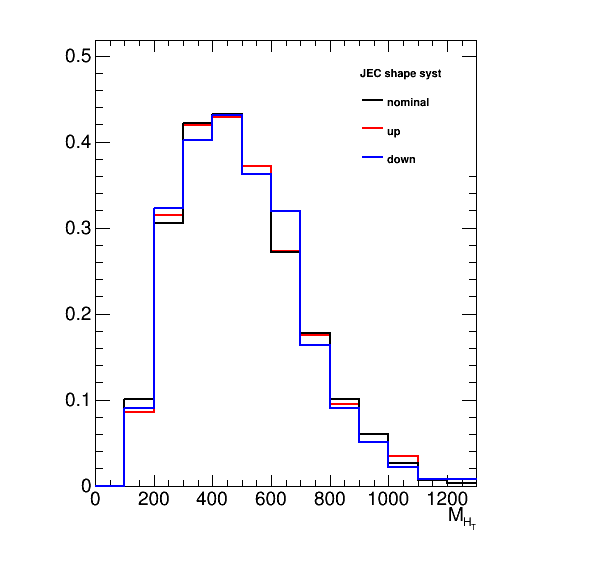
\includegraphics[width=0.5\textwidth]{figures/closureTests/mhtJetSyst_SMS_T1bbbb_2J_mGl1000_mLSP900_JEC_ge3b_ge5j_800_1600.png}
  \caption{\label{fig:jec-shape} Templates for the JEC shape systematic for $\geq$ 3 b-jets $\geq$ 5 jets and \scalht > 800 for the 10 \ifb luminosity scenario}
\end{figure}

\subsubsection{PDF uncertainties\label{sec:pdf-sets}}

\newcommand{\lcr}{Left: $\frac{\epsilon_{CTEQ6L1}}{\epsilon_{CT10}}$,
  center: $\frac{\epsilon_{CTEQ6L1}}{\epsilon_{MSTW08}}$, right:
  $\frac{\epsilon_{CTEQ6L1}}{\epsilon_{NNPDF2.1}}$}

The samples are produced with the \verb!CTEQ6L1! PDF set by
default. The shape is compared with that obtained with
three alternative PDF sets: \verb!CT10!, \verb!NNPDF2.1!, and
\verb!MSTW2008!. The envelope and its uncertainties are determined
following the PDF4LHC recommendation~\cite{pdf4lhc}.


\subsubsection{Initial state radiation\label{sec:sms-syst-isr}}
Will have to cook up a recipe for this\ldots


\subsubsection{\texorpdfstring{\mht/\met}{MHT/MET} cleaning cut\label{sec:sms-syst-mht-met}}
The efficiencies for the requirement $\mht/\met < 1.25$ must be measured in 
data and simulation as a function of \mht for each \scalht bin.
The ratio of these two efficiencies should be unity. Deviation from unity is taken
to represent the uncertainties on the simulation modelling of this
variable for processes with significant, genuine \met. This can be used
to define templates for the uncertainty on this quantity.

\subsubsection{Dead ECAL filter\label{sec:sms-syst-dead-ecal}}

The ratio of efficiencies observed in data and simulation for the dead
ECAL filter may be used as in Section~\ref{sec:sms-syst-mht-met} to templates
for the uncertainty from the Dead ECAL filter. 
